Sean las circunferencias $C_1$ y $C_2$ de redio $r$. Lea de la consola el radio $r$ (puede ser cualquier número real, no solo entero) y calcule el área sombreada.

\begin{center}
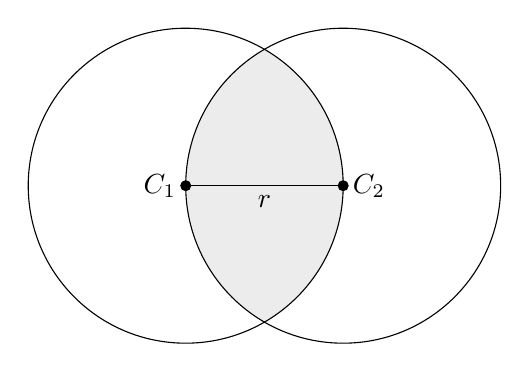
\begin{tikzpicture}
    % Definir el radio
    \def\r{2}

    % Sombrear el área de intersección
    \begin{scope}
        \clip (0,0) circle (\r);
        \fill[gray!15] (\r,0) circle (\r);
    \end{scope}

    % Dibujar la primera circunferencia
    \draw (0,0) circle (\r);

    % Dibujar la segunda circunferencia con un radio coincidente
    \draw (\r,0) circle (\r);

    % Marcar los centros de las circunferencias
    \fill (0,0) circle (2pt) node[left] {$C_1$};
    \fill (\r,0) circle (2pt) node[right] {$C_2$};

    % Dibujar el radio coincidente y etiquetarlo
    \draw (0,0) -- (\r,0) node[midway, below] {$r$};
\end{tikzpicture}
\end{center}

\subsection*{Ejemplos:}
\begin{itemize}
    \item Entrada: \texttt{3}\\
          Salida: \texttt{El área sombreada es: 18.84955592153876}
    \item Entrada: \texttt{5}\\
          Salida: \texttt{El área sombreada es: 52.35987755982988}
    \item Entrada: \texttt{10}\\
          Salida: \texttt{El área sombreada es: 209.43951023931953}
\end{itemize}
